% preamble
\documentclass{article}
\usepackage{fullpage}
\usepackage{fancyhdr}
\setlength{\headheight}{12pt}
\usepackage[headsep=1cm,total={6.5in, 8.5in}]{geometry}

% useful packages
\usepackage{amsmath,amssymb, amsthm}

% add your own packages here
\usepackage{verbatim}
% \usepackage[style=verbose]{biblatex}
\usepackage{enumitem}

\usepackage{tikz}
% \usepackage{filecontents}
% \begin{filecontents}{myreferences.bib}
%     @online{foo12,
%       year = {2012},
%       title = {footnote-reference-using-european-system},
%       url = {http://tex.stackexchange.com/questions/69716/footnote-reference-using-european-system},
%     }
% \end{filecontents}

% % Save the bib to disk (or update it).
% \addbibresource{myreferences.bib}

% commands for header, fill in the appropriate values
\newcommand{\codename}	{Snoop Matroidd} % type name here
\newcommand{\settitle}	{Set 5} %type set title here (ex. Problem Set 3, Midterm)
\newcommand{\latesub}	{No} % type yes/no indicating late submission

% a few helpful commands 
\newcommand{\RR}{\mathbb{R}} % typing \RR prints the Blackboard R used for Real Numbers
\newcommand{\NN}{\mathbb{N}} % typing \NN prints the Blackboard N used for Natural Numbers
\newcommand{\ZZ}{\mathbb{Z}} % typing \ZZ prints the Blackboard Z used for Integers

% construct your own commands here

\newcommand{\GCD}{\textrm{GCD}}

\newtheorem{theorem}{Theorem}[section]
\newtheorem{lemma}[theorem]{Lemma}

% commands for header, don't adjust
\begin{document}
\thispagestyle{empty}
\begin{center}
      \framebox[6.5in]{
            \vbox{
                  \vspace{2mm}
                  \makebox[6.3in][l]{\textbf{CS~38~~~Algorithms}\hfill \textbf{\today}}
                  \vspace{4mm}
                  \makebox[6.5in][c] {\Large \hfill \settitle{\hfill}}
                  \vspace{2mm}
                  \makebox[6.3in][l] {\textbf{Codename: } \codename{ \hfill \textbf{Late Submission:}
                              \latesub}}
                  \vspace{2mm}
            }
      }
\end{center}
\vspace*{1mm}
\pagestyle{fancy}\lhead{Codename: \codename} \chead{\settitle}
\rhead{\today}

% insert solution here
\section{Problem 1 (6 points)}
Collaborated with: No One

\subsection{Proposition}


\begin{enumerate}[label= (\alph*)]
      \item Consider the frequences (as percentages) for a set of characters. (There are
            in fact real frequencies for russian language text, as taken from
            practicalcryptography.com We have rewritten them here with unrelated greek letters
            for ease of \LaTeX{}ing).

            Design an optimal Huffman code. Show for the first five steps, how you
            assembled the code.

      \item In class we mentioned that the greedy strategy of assembling a prefix-free
            code for an alphabet \(\Sigma \), is optimal only if the encodings of ''0''
            and ''1'' are equal cost (in terms of space storage, or transmission time). No
            polynomial-time algorithm is known for designing optimal prefix-free codes
            when the encodings have different costs.

            \paragraph{} Suppose the cost of encoding a ''0'' is \(w_0 > 0\), and ''1'' is
            \(w_1 < 0\), with \(w_0 < w_1\). Consider the following generalization of
            Huffman's greedy algorithm. We always work with ``virtual characters'', which
            are subsets \(S \subseteq \Sigma \) and have frequency \(p_S = \sum_{a\in
                  S}p_a\). Each virtual character is encoded with a tree, with the characters at
            the leaves, and bits labeling the edges. Initially, every virtual character is
            simply a singleton set consisting of one character from the alphabet; and it is
            encoded with the tree consisting solely of a root vertex.
            \paragraph{} The algorithm is to repeatedly pick the two lowest-frequency
            virtual characters, say \(S, T\) with \(p_S leq p_T\), eliminate them and
            replace them by the virtual character \(S \cup T\); the two trees are merged
            by installing a new root, from which an edge labeled ''0'' leads to \(S\) and
            an edge labeled ''1'' leads to \(T\). This continues until all characters are
            leaves of a single tree. The prefix-tree encoding of a character is simply the
            sequence of bits on the simple path from the root to that leaf.
            \paragraph{} Show by specific example (choose \(w_0\) and \(w_1\), and an
            alphabet with associated frequency counts) that this can result in a
            sub-optimal prefix-free code. (You don't have to look far. There is an example
            with \(|\Sigma| = 4\).)
\end{enumerate}

\subsection{Part (a)}


\subsection{Part (b)}
\subsubsection{Algorithm}
\begin{enumerate}
      \item
\end{enumerate}

\subsubsection{Proof of Correctness}


\subsubsection{Complexity Analysis}


\newpage
\section{Problem 2 (6 points)}
Collaborated with: No Collab

\subsection{Proposition}
Design and analyze an algorithm that takes an input an undirected graph \(G=(V,E)\) and
determines whether G contains a simple cycle (that is, a cycle with no repeated vertices)
of length 4. (Following our usual convention, an undirected graph does not have loops or
multiple edges.) Its running time should be at most \(O(|V|^2)\). (Or \(O(|V|^3)\) for
partial credit.)

\subsection{Algorithm}
\begin{enumerate}
      \item Our algorithm operates on a list of edges for every vertex \(v \in V\). It will return
            True if the graph contains a 4 cycle, and False if not. It works by looping
            over every vertex and checking the adjacency lists of the vertices adjacent to
            it and checking if there is a cycle if a cycle form exists in the resulting
            data structure.\footnote{TA Notes 6.1.4}
      \item First convert our vertex input into adjacency list form if it is not already.
      \item Let \(V' = V\) if \(V\) is already an adjacency list, else initialize it to an
            empty list. For every vertex \(v \in V\): \begin{enumerate}
                  \item Add an entry in \(V'\) for \(v\).
                  \item Add each vertex that shares an edge with \(v\) to \(V^{\prime}[v]\).
            \end{enumerate}

      \item For every vertex \(v \in V^{\prime}\): \begin{enumerate}
                  \item Let \(2^\prime \) be an array of size \(|V^{\prime}| \)
                        initialized to ''0''s.
                  \item For each vertex \(x \in V^{\prime}[v]\): \begin{enumerate}
                              \item For each vertex \(y \in V^{\prime}[x]\): \begin{enumerate}
                                          \item If \(2^\prime [y] = 1\) AND \(y \neq v\), Return True.
                                          \item Else,  set \(2^\prime [y] = 1\).
                                    \end{enumerate}
                        \end{enumerate}
            \end{enumerate}
      \item Return False.
\end{enumerate}

\subsection{Proof of Correctness}
\begin{proof} The above algorithm decides whether a graph contains a cycle of length 4.
      \begin{enumerate}
            \item Each 4-cycle takes a form that matches this drawing where \(First \neq Second\),
                  \(Fourth \neq Third\), and
                  \(Second \neq Fourth\):
                  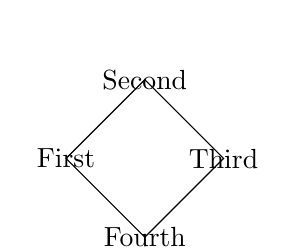
\begin{tikzpicture}
                        \node (a) at (0,0) {First };
                        \node (b) at (1,1) {Second };
                        \node (c) at (2, 0) {Third};
                        \node (d) at (1, -1) {Fourth};
                        \draw (a.center) -- (b.center) -- (c.center) -- (d.center) -- cycle;
                  \end{tikzpicture}
            \item In this class we don't deal with graphs that have multiple edges between
                  vertices or that contain self-loops, so our algorithm doesn't need to
                  consider the cases where Second or Fourth may be First itself in the
                  cycle.\footnote{TA Notes 6.1.1}
            \item Thus, if the same vertex shows up in the adjacency list of any vertex
                  more than once, there must be two paths between a vertex and the one added to
                  the list twice, and thus a 4 cycle of the form above exists and returns
                  correctly.
            \item If the algorithm walks the entire adjacency list for every vertex
                  in the graph and had not attempted to add any entries twice, then we
                  have checked the entire graph and none were found, so we correctly
                  return False.
      \end{enumerate}
\end{proof}

\subsection{Complexity Analysis}
\begin{proof} The runtime is \(O(|V|^2)\).
      \begin{enumerate}
            \item Converting the graph to an adjacency list in step 3 takes at most
                  \(O(|V|^2)\) time.
            \item The loop at step 4 runs for at most \(|V|\) iterations.
            \item Each iteration of the loop constructs a list of length \(|V|\) in time \(O(|V|)\).
            \item The innermost loop at \(4.b.i\) can reach \(v\) at most \(|V|\) times,
                  and will check each vertex once.
            \item The algorithm has a whole thus has to perform \(2 *|V| + 1 |V'[y]|\)
                  checks.
            \item Thereforce the runtime of this algorithm is in \(O(|V|^2)\).
      \end{enumerate}

\end{proof}

\newpage
\section{Problem 3 (6 points)}
Collaborated with: No One

\subsection{Proposition}
Let \(G=(V,E,w)\) be a weighted graph with \(n\) vertices \(m\) edges. Define the
\textit{bottleneck distance} between two vertices as follows:
\[g(x,y) = \min \{ h(p) : p \text{ is a path from } x \text{ to } y \} \]
where \(h(u_o,\ldots,u_k) = \max \{ w(u_{j-1}, u_j) : j=1,\ldots,k \} \).

Give an \(O(m +  n \log (n))\)-time algorithm that computes the bottleneck distance
between two given vertices in a directed weighted graph.

You may rely on the fact (which is covered in the TA notes and in Ch. 19 of CLRS), that
using Fibonacci heaps rather than binary heaps, Dijkstra's algorithm runs in time \(O(m +
\log n)\).

\subsection{Algorithm}
\begin{enumerate}
      \item We will use a modified form of Dijsktra's Algorithm\footnote{TA Notes 6.3.1}.
      \item Using this algorithm from the notes as a base, modify the update rule for the priority queue
            to ``Decrease key of x to \(- \infty \)'', for the input to \(x\) to \(g(x, y)\).
      \item Let \(G = (V, E, w)\) be a directed graph with \(w, x \in V\).
      \item Generate a priority queue \(P\) and push onto \(P\) every element \(v \in V\) with key
            \(\infty \).
      \item Decrease key of \(x\) to \(- \infty \).
      \item While P isn't empty: \begin{enumerate}
                  \item Pop and mark the min weight element from \(P\); call it \(a\).
                  \item For every unmarked vertex \(b\) s.t. \( (a,b) \in E\), if
                        \(key(b) > \max \{ w(a,b), key(a) \} \): \begin{enumerate}
                              \item Decrease key of \(b\ to \max \{ w(a,b), key(a) \} \).
                              \item Set \(parent(b) \leftarrow a\).
                        \end{enumerate}
                  \item Set \(g(x, a) \leftarrow key(a)\)
            \end{enumerate}
      \item Return \(g(x,y)\).
\end{enumerate}

\subsection{Proof of Correctness}
\begin{proof} \(g(x,y)\) is a correct implementation of bottleneck distance
      \begin{enumerate}
            \item We will follow a similar proof to the proof that \(dist(u, *)\) is the
                  correct distance function using induction.\footnote{TA Notes 6.3.2}
            \item Assume that \(g^\prime (x,*)\) is the correct bottleneck distance function.
            \item Base case: \(g(x,x)\) \begin{enumerate}
                        \item \(key(x)\) will initially be set to \(-\infty \) and never be set.
                        \item Thus \(g(x,x) = g^{\prime}(x,x) = -\infty \).
                  \end{enumerate}
            \item Observe that the bottleneck distance won't be decreased by cycles.
            \item Inductive Assumption: \(g^{\prime}(x,y) \leq g(x,y) \forall y \in V\)
                  \begin{enumerate}

                        \item Let \(z\) be the vertex returned from the queue where
                              \(g^{\prime}(x, z) < g(x,
                              z)\).
                        \item   Let \(Z\) be the set of vertices popped off the queue
                              prior to \(z\).
                        \item Since we know \(g^{\prime}(x,z)\) is the correct bottleneck
                              distance path function, we can also observe that the
                              weightiest edge along the path must have the minimum
                              possible weight in traversing from \(x\) to \(z\).
                        \item To determine its a bottleneck we need to know the maximum
                              weighted edge to determine he bottleneck, which is either
                              previously computed or is the next weight to check.
                        \item Since we assume prior iterations were computed correctly,
                              then we can compute the path from \(x\) to the next element
                              \(m\).
                        \item Therefore the decrease in the key after popping the final
                              element \(y\) will set \(g^{\prime}(z,m) = g(z, m)\).
                        \item Assume that \(z \neq m\), such that \(z\) was popped from \(m\).
                        \item Contradiction! \(g(x, z) = key(z) < key(m) < key(z)\).
                        \item Thus we have proven the bottleneck distance function we
                              implemented is correct.
                  \end{enumerate}
      \end{enumerate}

\end{proof}

\subsection{Complexity Analysis}
\begin{proof} This algorithm runs in \(O(m + n \log (n))\) time.\begin{enumerate}
            \item We already know Dijkstra's Algorithm can fun in \(O(m + n \log (n))\)
                  time using Fibonacci heaps.\footnote{TA Notes 6.3.3}
            \item Our only change was swapping the update rule to a constant time
                  maximimizing comparison.
            \item Therefore the runtime is unchanged and remains \(O(m + n \log (n))\).
      \end{enumerate}

\end{proof}
\newpage


\section{Problem 4 (6 points)}
Collaborated with: No One

\subsection{Proposition}
\paragraph{}

\begin{enumerate}[label= (\alph*)]
      \item Now assume that the graph G is undirected and unconnected. Show that the bottleneck
            distance \(g(x,y)\) does not change if we reduce the set of edges to a mininum spanning
            tree.
      \item Give an \(O(n^2)\)-time algorithm for the all-pairs bottleneck distance
            problem in an undirected graph.
\end{enumerate}
\subsection{Part A}
\begin{proof} The bottleneck
      distance \(g(x,y)\) does not change if we reduce the set of edges to a mininum spanning
      tree.
      \begin{enumerate}
            \item Let \(G\) be a undirected and connected graph.
            \item Let \(T\) be a minimimum spanning tree formed from \(G\).
            \item Assume for the sake of contradiction that the bottleneck distance did
                  change if we reduced the set of edges to a minimum spanning tree.
            \item If it did, then there must exist a path \(p^\prime \) from \(x\) to
                  \(y\) that has a edge weight equal to the bnottleneck that is not in the
                  minimum spanning tree \(T\).
            \item Since \(T\) is a spanning tree there must be another unique path \(p\) from \(x\) to \(y\).
            \item If we remove the edge with the greatest weight from \(p\), we have split
                  the tree into two sub trees connected at the edge we removed.
            \item We know that the hypothetical path \(p^\prime \) must also connect the
                  vertices \(x\) and \(y\).
            \item Thus there must be some edge that can be connected also reconnect
                  our subtrees back into a spanning tree.\item Because we know
                  \(p^\prime \) has an equal edge weight to the bottleneck distance, we
                  also know that this was the minimum weight, as we took the edge with the
                  highest weight along \(p\).
            \item Any such edge that could be connected however would produce a spanning
                  tree that is a lower weight than \(T\), meaning \(T\) wasn't a minimum
                  spanning tree.
            \item Contradiction! Therefore the path with the bottleneck distance as its
                  edgeweight must be part of a minimum spanning tree.
            \item Thus the bottleneck distance does not change if we reduce to an Mininum
                  Spanning Tree.
      \end{enumerate}
\end{proof}

\subsection{Part B}
\subsubsection{Algorithm}
\begin{enumerate}
      \item Let \(T = (V, F )\) be a MST returned by Prim's algorithm\footnote{TA
            Notes 5.8.1} (Runtime \(O(m + n \log n)\)).
      \item Let all vertices be considered unmarked to begin with.
      \item Let \(H be the set of directed edges over F towards both vertices\).
      \item Let \(v\) be the first vertex selected from the graph \(G\) in some manner.\begin{enumerate}
                  \item Let \(Q\) be initialized as a First In First Out queue.\footnote{TA Notes 6.2.3}
                  \item Set \(g(v,v) = -\infty \).
                  \item Mark \(v\) and push it into \(Q\).
                  \item While Q is not empty:\begin{enumerate}
                              \item Pop a vertex from \(Q\); call it \(a\).
                              \item For every vertex \(b\) st. \(a, b \in H\), if \(b\) is unmarked.
                                    \begin{enumerate}
                                          \item Mark \(b\) and push \(b\) onto \(Q\).
                                          \item Set \(parent(b) \leftarrow a\).
                                          \item Set \(g(v, b) \leftarrow \max \{ g(v,a) , w(a,b) \} \)
                                    \end{enumerate}
                        \end{enumerate}
            \end{enumerate}
      \item Repeat the prior step for all remaining vertices in \(v \in V\).
      \item Return the resulting values of \(g(x,y)\).
\end{enumerate}

\subsubsection{Proof of Correctness}
\begin{proof}
      \begin{enumerate}
            \item Prim's algorithm is given as correct in the TA Notes\footnote{TA Notes 5.8.1}
            \item We proved in part (a) that reducing the graph's edges to a minimum
                  spanning tree does not change the bottleneck distance.
            \item We will prove our modification to Breadth First Searc\footnote{TA Notes
                        6.2.5} are correct using induction on the tree's depth.
            \item Base Case: Tree depth of 0 \begin{enumerate}
                        \item In this case there is only the root node, and the bottleneck
                              distance is the initial value \(-\infty \).
                  \end{enumerate}
            \item Inductive Case:  d > 0\begin{enumerate}
                        \item At each level of BFS we explore one depth \(d\) of the tree.
                        \item We know that given the MST that each path between vertices
                              must be unique, and when we find the bottleneck distance we
                              know there must only be this unique path.
                        \item Therefore the bottleneck distance is the maximum weight edge
                              along the path \(p\).
                        \item If all the prior depths are correct for our inductive
                              hypothesis.
                  \end{enumerate}
      \end{enumerate}
\end{proof}

\subsubsection{Complexity Analysis}
\begin{proof}
      \begin{enumerate}
            \item
      \end{enumerate}
\end{proof}

\end{document}